% Interest of the model
Comme mentionné précédemment, à cause de la complexité du système il est préférable pour cette étude de considérer un sytème modèle. Dans cette section, nous décrivons le modèle et ses caractéristiques, avant de détailler sa construction, et de discuter des simulations dans lesquelles il intervient.

% Description
    \subsection{Description du modèle}

Le système modèle est composé d'électrodes en graphites immergées dans un électrolyte aqueux d'hydroxyde de sodium, sa structure est présentée à la \autoref{fig:schema_structure} et ses caractéristiques au \autoref{tab:caracteristiques_systeme}.

\begin{figure}[h!]
    \centering
    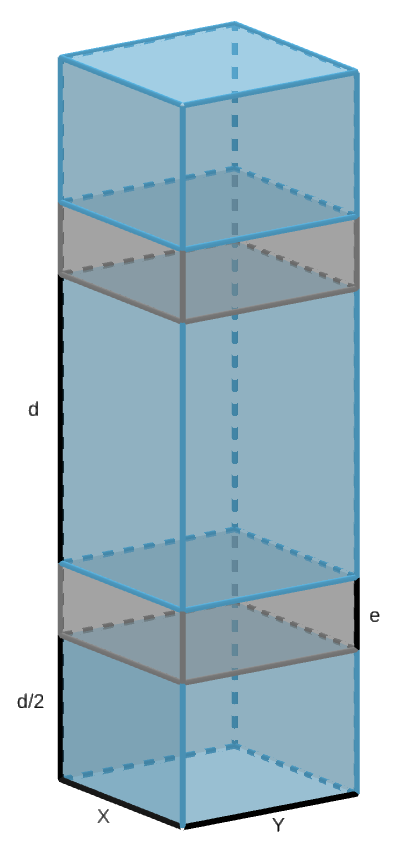
\includegraphics[height = 5 cm]{schema_structure.png}
    \caption{Schéma de la structure du système modèle}
    \label{fig:schema_structure}
\end{figure}

\begin{table}[h!]
    \centering
    \begin{tabular}{l || l | l l}
        \hline
        Groupe &Caractéristique &Valeur &\\
        \hline
        Système &Dimensions &$(22.104, 21.270, \sim 40)$ &\unit{\angstrom}\\
        &Particules &$\sim \num{3000}$ &\\
        \hline
        Électrodes &Séparation &$\sim \num{20}$ &\unit{\angstrom}\\
        &Atomes (par électrode) &\num{540} &\\
        \hline
        Électrolyte &Molécules d'eau &\num{314} &\\
        &Concentration &$\sim \num{1.0}$ &\unit{\mole \per \liter}\\
        &Ions &\num{6} &\\
        \hline
    \end{tabular}
    \caption{Caractéristiques du système}
    \label{tab:caracteristiques_systeme}
\end{table}

% Construction
    \subsection{Construction du modèle}

\begin{figure}[h!]
    \centering
    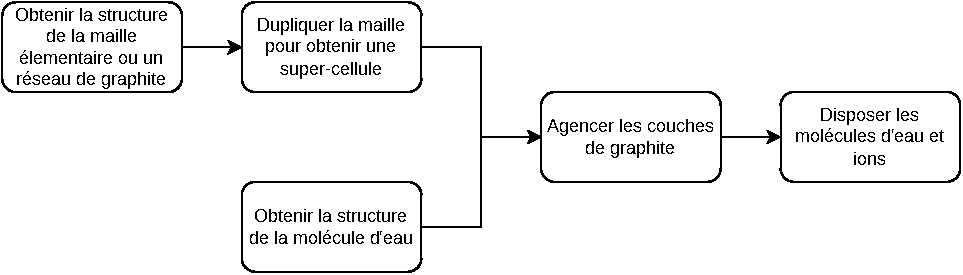
\includegraphics[height = 3 cm]{construction_structure.pdf}
    \caption{Démarche de construction de la structure}
    \label{fig:construction_structure}
\end{figure}

Pour construire la structure du modèle, la démarche \autoref{fig:construction_structure} a été adoptée afin d'obtenir le système aux dimensions et caractéristiques désirées, avec une configuration initiale des particules convenable.

\textbf{Obtention des structures}\\
Les données sur les structures des molécules ont été obtenues grâce à la \href{http://www.crystallography.net/cod/}{Crystallography Open Database} (COD) et celles-ci sont présentées à la \autoref{fig:molecules_initiales}.

\begin{figure}[h!]
	\centering
	\begin{subfigure}[t]{.49\textwidth}
		\centering
		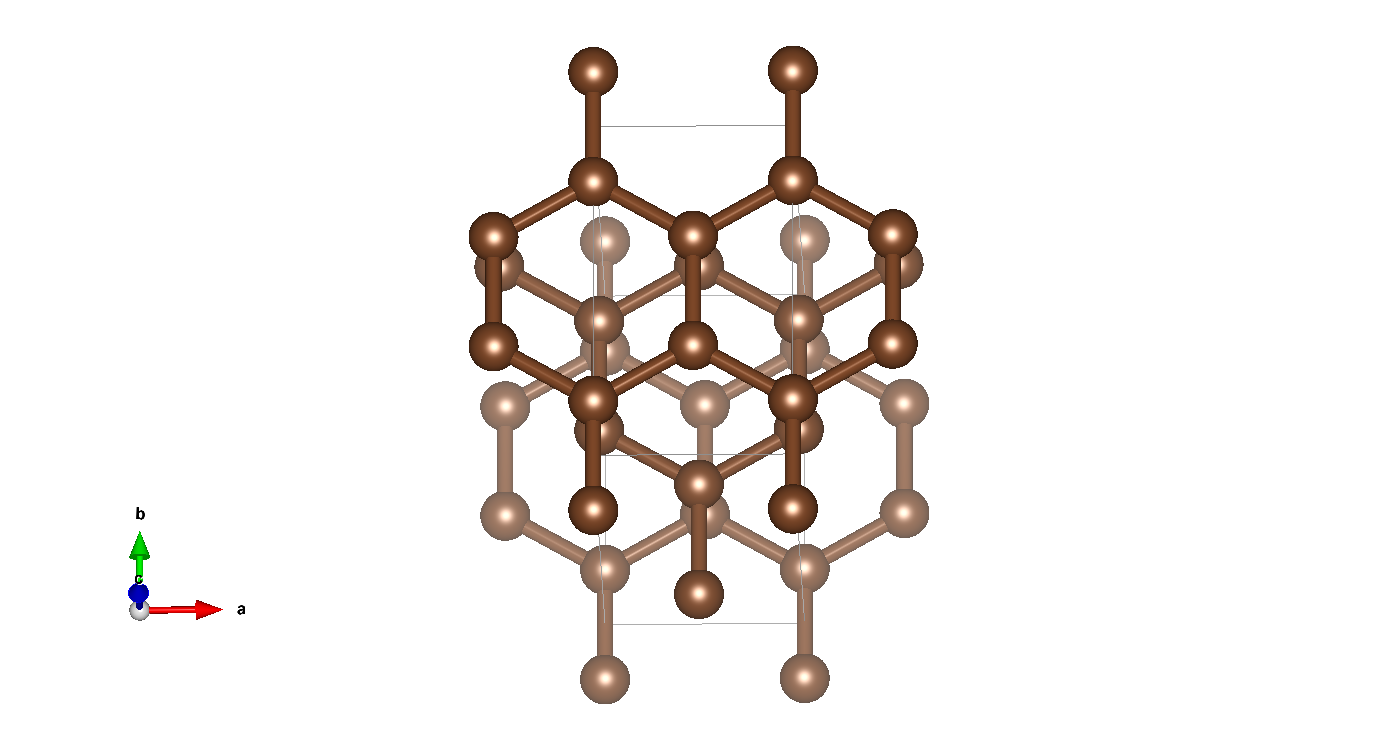
\includegraphics[width = \textwidth]{graphite.png}
		\caption{Réseau de graphite}
	\end{subfigure}%
    ~
	\begin{subfigure}[t]{.49\textwidth}
		\centering
		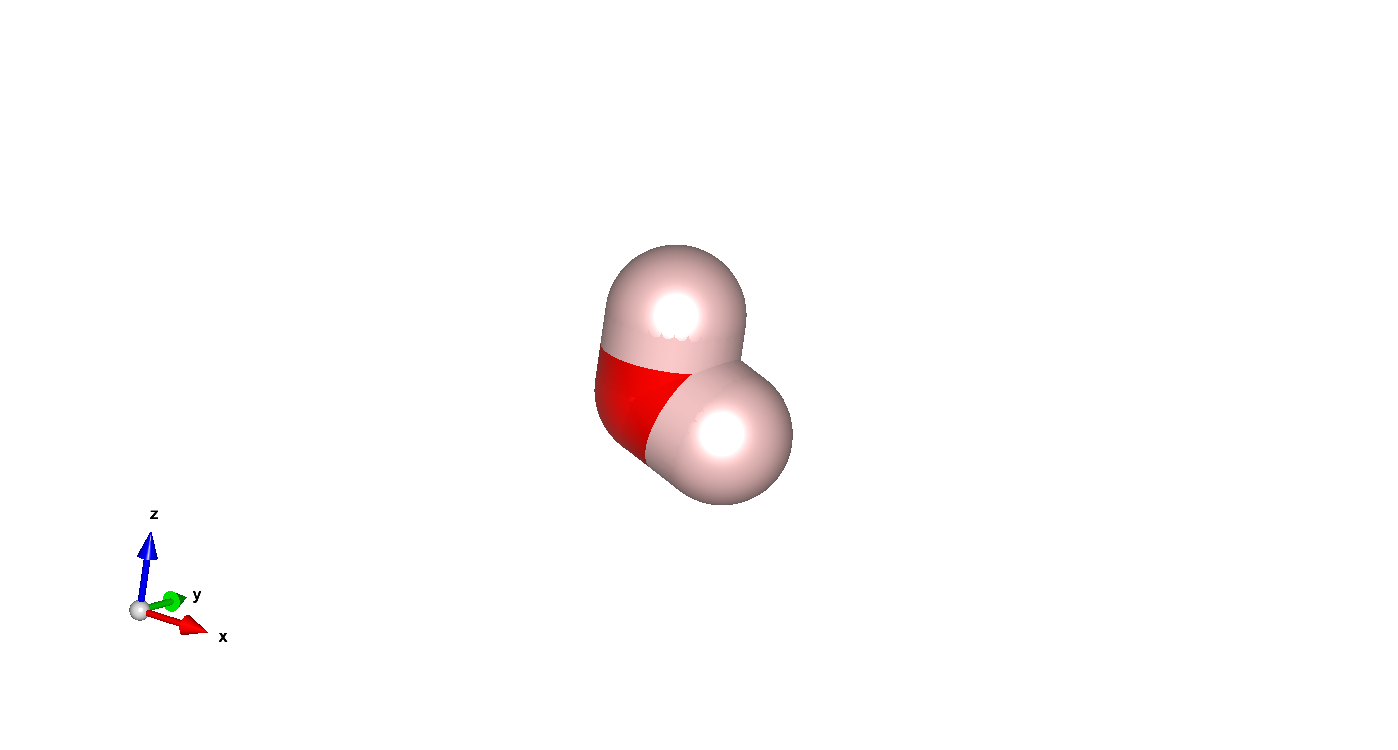
\includegraphics[width = \textwidth]{water.png}
		\caption{Molécule d'eau}
	\end{subfigure}
	\caption{Structures des molécules provenant de la COD}
	\label{fig:molecules_initiales}
\end{figure}

\textbf{Obtention de la super-cellule}\\
La structure de graphite de base a pu être étendue grâce à un logiciel tier\cite{momma_vesta_2011}, \num{9} fois selon la direction $[OX)$ et \num{5} fois selon la direction $[OY)$ afin que les dimensions dans ces directions soient du même ordre, pour obtenir une électrode de graphite (\autoref{tab:dimensions_structures} et \autoref{fig:electrode}).

\begin{table}[h!]
    \centering
    \begin{tabular}{l | c c c}
        \hline
        Structure &X [Å] &Y [Å] &Z [Å]\\
        \hline
        Graphite de base &\num{2.456} &\num{4.254} &\num{6.696}\\
        Électrode de graphite &\num{22.104} &\num{21.270} &\num{6.696}\\
        \hline
    \end{tabular}
    \caption{Dimensions des sctructures}
    \label{tab:dimensions_structures}
\end{table}

\begin{figure}[h!]
    \centering
    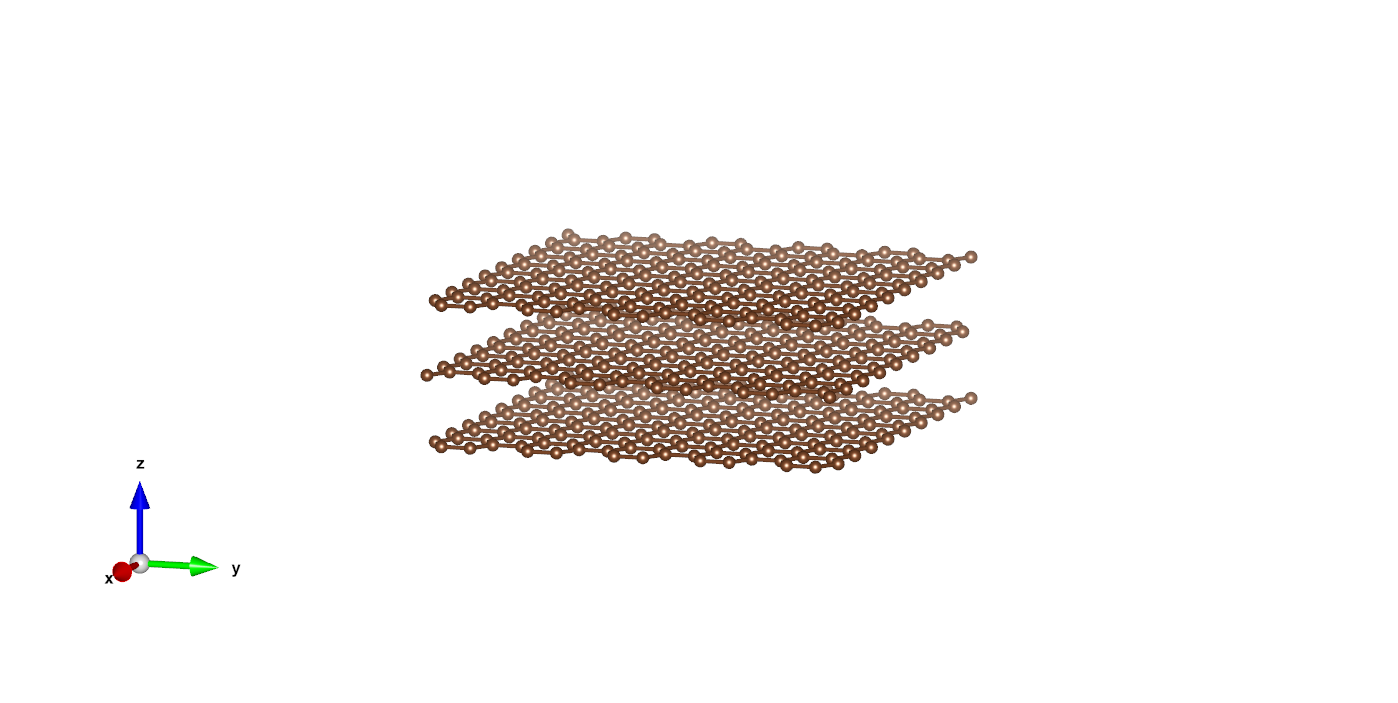
\includegraphics[height = 5 cm]{electrode.png}
    \caption{Électrode obtenue après duplication du réseau de graphite}
    \label{fig:electrode}
\end{figure}

\textbf{Agencement des particules}\\
Les particules ont pu être disposées pour construire le modèle à l'aide de \packmol{}\cite{martinez_packmol_2009}, détails à l'\autoref{apdx:packmol}.

Pour obtenir des configurations initiales suffisamment stables nous avons choisi de répartir les entités en les séparant d'au moins \qty{2.5}{\angstrom} : entre les molécules et ions de l'électrolyte, et entre les particules de l'électrolyte et les électrodes.\\
Et pour respecter les conditions aux limites périodiques, cette séparation a également été appliquée aux bords du système : nous ajoutons un retrait égal à la moitité de cette séparation à chaque bord.

Finalement, nous obtenons la configuration présentée à la figure \autoref{fig:structure_finale}.

\begin{figure}[h!]
    \centering
    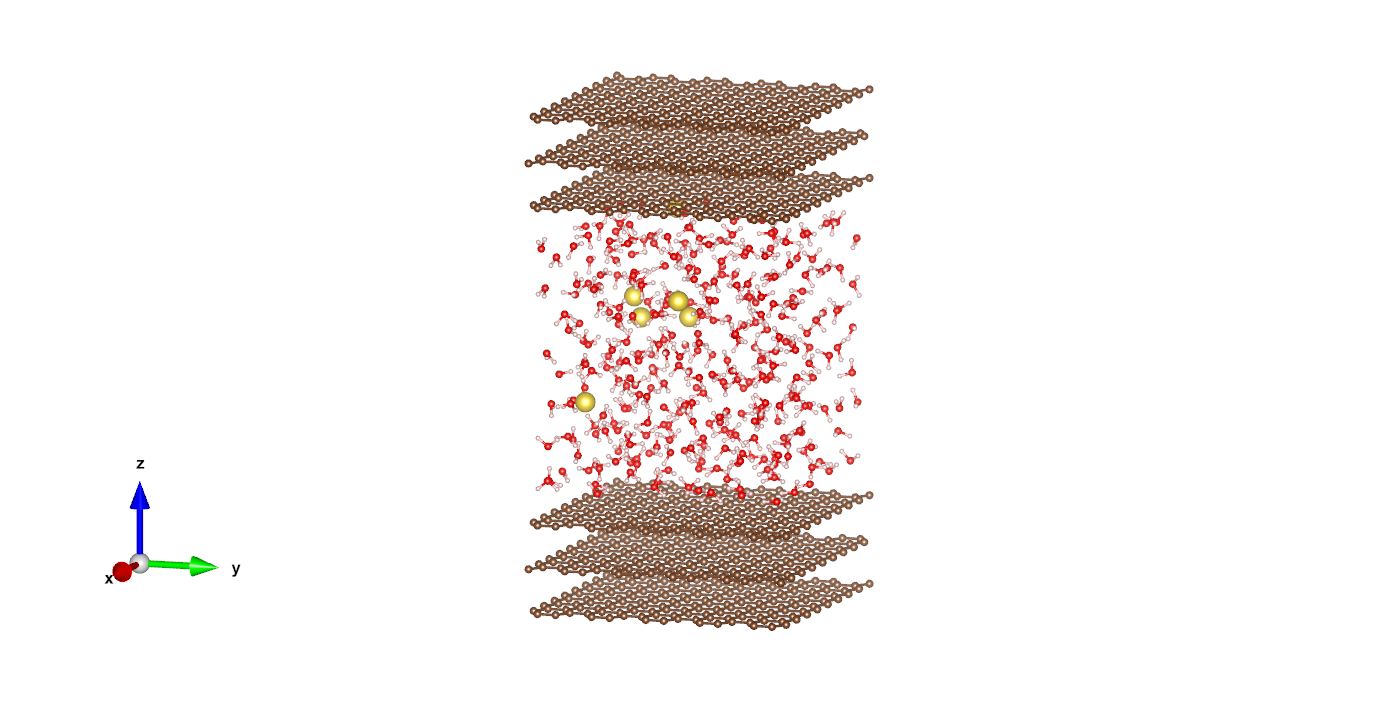
\includegraphics[height = 5 cm]{structure.png}
    \caption{Structure finale obtenue après agencement des molécules}
    \label{fig:structure_finale}
\end{figure}

% Simulations details
    \subsection{Déroulement et détails des simulations} \label{sec:deroulement_simulations}

\begin{table}[h!]
    \centering
    \begin{tabular}{l || l | l l}
        \hline
        Étape &Paramètre &Valeur &\\
        \hline
        Toutes &\lstinline!timestep! &\num{0.1} &\unit{\femto \second}\\
        &potentiel &\reaxff{} &\\
        \hline
        Minimisation &\lstinline!maxiter! &\num{1000} &\\
        &\lstinline!maxeval! &\num{10000} &\\
        &\lstinline!etol! &\num{e-05} &\\
        &\lstinline!ftol! &\num{e-06} &\unit{\kilo \cal \per \mole \per \angstrom}\\
        \hline
        Relaxation et Stabilisation &durée &\num{200000} &\\
        & &\num{20.0} &\unit{\pico \second}\\
        &\lstinline!T_target! &\num{300.0} &\unit{\kelvin}\\
        &\lstinline!P_target! &\num{1.0} &\unit{\atm}\\
        \hline
        Simulation &durée &\num{10000000}\\
        &polarisation &\echemdid{} &\\
        & &\num{1.0} &\unit{\nano \second}\\
        &\lstinline!T_target! &\num{300.0} &\unit{\kelvin}\\
        \hline
    \end{tabular}
    \caption{Récapitulatif des paramètres des simulations}
\end{table}

\begin{figure}[h!]
    \centering
    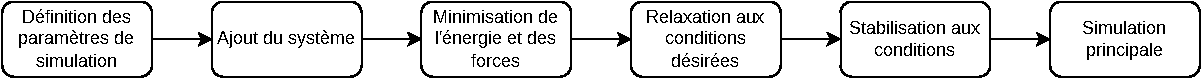
\includegraphics[width = \textwidth]{deroulement_simulations.pdf}
    \caption{Déroulement des simulations}
    \label{fig:deroulement_simulations}
\end{figure}

Toutes les simulations suivent le déroulement de la \autoref{fig:deroulement_simulations} afin de définir les paramètres de simulation, de préparer le système, et de lui permettre de s'équilibrer.

\textbf{Paramétrisation}\\
Elle consiste à définir les paramètres clés de la simulation. Par exemple :
\begin{itemize}
    \item le pas de temps (\lstinline!timestep!) sélectionné pour les simulations est de \qty{0.1}{\femto \second}
    \item les interactions sont basés sur le potentiel réactif \reaxff{} (détaillé à la \autoref{sec:reaxff})
    \item la mise en place de la différence de potentiel entre les électrodes est réalisée grâce à \echemdid{} (détaillé à la \autoref{sec:echemdid})
\end{itemize}

\textbf{Ajout du système}\\
Ceci est effectué avec une commande \lammps{} de lecture de données. Pour ce faire, il est nécessaire de convertir les données des positions des particules du système (détails à la \autoref{sec:systeme_modele}) en données \lammps{} (détails à l'\autoref{apdx:conversion_lammps}).

\textbf{Minimisation}\\
Cette étape est essentielle au démarrage d'une simulation : elle sert à s'assurer que la configuration de départ de la simulation soit "correcte" et que le système soit stable.

Elle consiste à déplacer les particules du système sans dynamique de manière à minimiser l'énergie potentielle et les forces totales du système. Cette procédure suit un algorithme de gradient conjugué avec pour fonction objectif l'énergie potentielle totale :
\begin{equation*}
    E(r_1, \dots, r_N) = \sum_{i, j} E_{pair} (r_i, r_j) + \dots + \sum_{i, j} E_{fix} (r_i)
\end{equation*}
où sont prises en compte les énergies : des interactions de paires, des liaisons et angles si présents, des interactions \textit{improper} ou \textit{dihedral}, et des \lstinline!fix! imposés lors de la minimisation (ex : ajout de contraintes, de forces appliquées sur les atomes, etc.).

\textbf{Relaxation et stabilisation}\\
Ces étapes utilisent un thermostat et barostat de Nosé--Hoover pour atteindre les conditions physiques recherchées et les stabiliser.

Les conditions de pression et de température recherchées sont $T = \qty{300}{\kelvin}$ et $P = \qty{1}{\atm}$, et les évolutions des quantités thermodynamiques lors de ces étapes sont typiquement celles des \autoref{fig:allures_thermostat_barostat}.

\begin{figure}[h]
    \centering
    \begin{subfigure}[t]{.49\textwidth}
        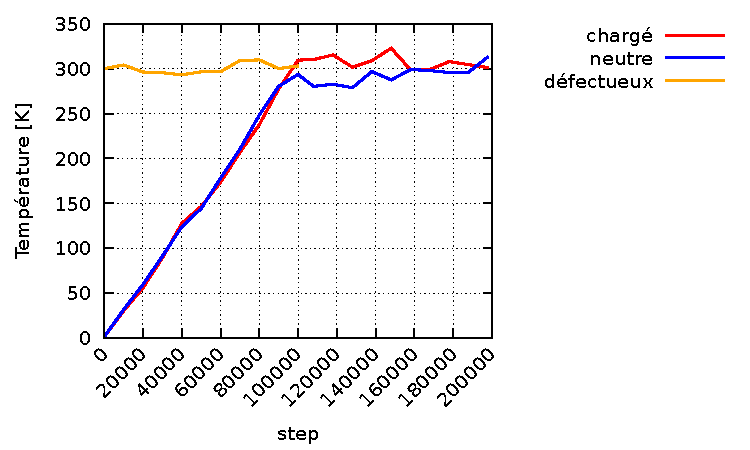
\includegraphics[width = \textwidth, draft]{relaxation_temp.pdf}
        \caption{Température}
    \end{subfigure}%
    ~
    \begin{subfigure}[t]{.49\textwidth}
        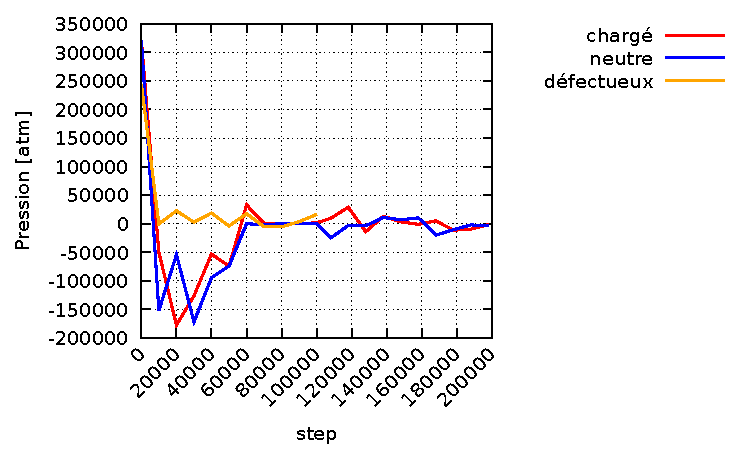
\includegraphics[width = \textwidth, draft]{relaxation_press.pdf}
        \caption{Pression}
    \end{subfigure}
    \begin{subfigure}[t]{.49\textwidth}
        \includegraphics[width = \textwidth, draft]{relaxation_density.pdf}
        \caption{Densité}
    \end{subfigure}
    \caption{Allures des grandeurs thermodynamiques pendant de la relaxation et la stabilisation {\tiny (chaque étape a lieu en \num{100000} \lstinline!timestep!s soit \qty{10}{\pico \second})}}
    \label{fig:allures_thermostat_barostat}
\end{figure}

\textbf{Simulation}\\
Cette étape sert à récolter des données et informations sur le système après qu'il a atteint l'équilibre.

Elle se déroule avec un thermostat de Nosé--Hoover à \qty{300}{\kelvin} et pour une durée $\geq~\qty{1}{\nano \second}$ (\autoref{fig:allures_simulation_principale}).

\begin{figure}[h]
    \centering
    \begin{subfigure}[t]{.49\textwidth}
        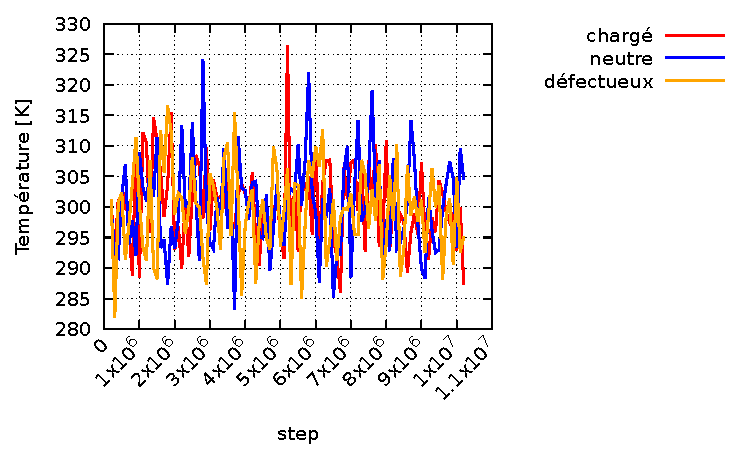
\includegraphics[width = \textwidth, draft]{main_temp.pdf}
        \caption{Température}
    \end{subfigure}%
    ~
    \begin{subfigure}[t]{.49\textwidth}
        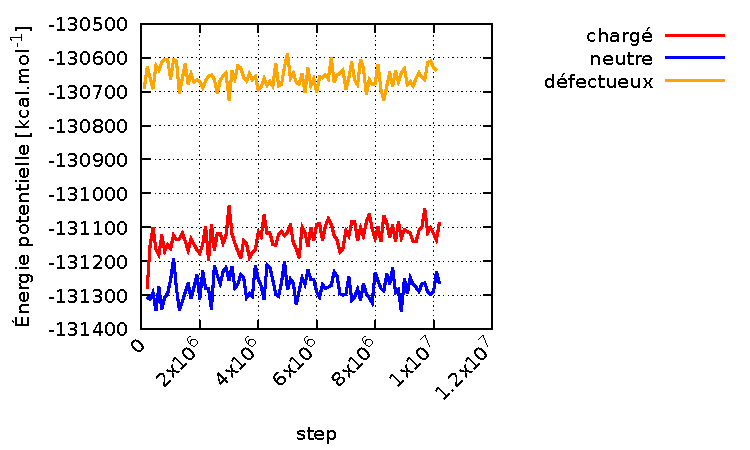
\includegraphics[width = \textwidth, draft]{main_epot.pdf}
        \caption{Énergie potentielle}
    \end{subfigure}
    \begin{subfigure}[t]{.49\textwidth}
        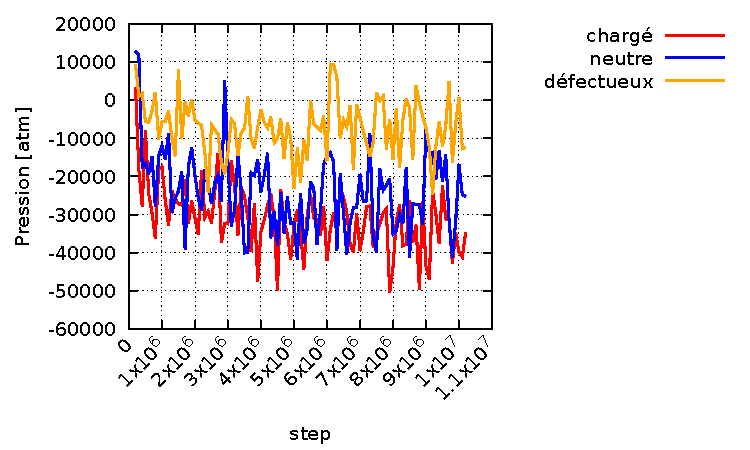
\includegraphics[width = \textwidth, draft]{main_press.pdf}
        \caption{Pression}
    \end{subfigure}
    \caption{Allures des grandeurs thermodynamiques pendant la simulation principale}
    \label{fig:allures_simulation_principale}
\end{figure}
